\section{Grasping and Manipulation}
\label{sec:manip}
%
Introduce LBR iiwa + Velvet Fingers 2 Gripper
%
\subsection{Grasp Planning}
\label{subsec:grasp_planning}
\begin{figure*}[t!] 
   \centering
    %\def\svgwidth{200pt} 
    \input{figs/grasp_interval.pdf_tex} 
   \caption{\textit{Grasp interval:} (Left) todo ... (Right) truncated grasp interval ...} 
   \label{fig:grasp_interval}
\end{figure*}

\cite{Bohg14}(data driven grasping) (SotA autonomous grasping systems) \cite{Pas13} cylinder shell
fitting

The key challenge for many applications of robotic mobile manipulation is autonomous grasping in
uncertain real-world environments. Finding collision-free trajec- tories leading the gripper-arm
chain from a given initial to a reachable final state (grasp planning together with vehicle and
manipulator motion planning) constitutes the fundament for any robot manipulation system. Currently,
despite of a large research effort, no commercially viable solution is available for this
problem. In today’s state-of-the-art autonomous grasping systems~\cite{Bere07, Srin10, Krug14a},
grasp planning and motion planning are usually seen as independent sub-problems~\cite{Dian10}. A
database storing object models together with pre-computed grasps is used to relax the need to find
suitable gripper poses/configurations~\cite{Mill04, Gold11, Krug14a}. In the online stage, sampling
based planners~\cite{LaVa06} attempt to generate valid trajectories for the pre-planned grasps,
which are executed in a feasible-first manner~\cite{Bere07}. During the execution phase, such
approaches necessitate many futile motion planning attempts, which often incurs significant time
delays since sampling based planners suffer from the curse of dimensionality. Also, while being able
to solve complicated planning problems if given enough time, these planners don’t scale well to
geometrically simple scenarios~\cite{Ratl09} and they are ill suited to incorporate contact events
with the environment.

 Instead of representing grasps as discrete gripper wrist poses and joint
configurations, we use grasp interval regions as depicted in Fig.~\ref{fig:grasp_interval}. These
grasp intervals can easily be transcribed as target tasks for the manipulator motion control and
allow for redundancy in the manipulator wrist positioning which eases reach-to-grasp
acquisition. Grasp interval formulation depends on the specific target object and has to be verified
experimentally. For now, we constrain ourselves to cylindrical objects as shown in
Fig.~\ref{fig:grasp_interval}. We then rely on the inherent capabilities of the grasping device and
the compliance of the system for successful grasp execution as stated below.


\cite{Bala12}(Identifying grasp principles from humans) \cite{Gien08a, Gien08b, Vahr10}(Task maps with RRT)
%
\subsection{Manipulator Motion Generation}
\label{subsec:manip_motion}
%
 \cite{Sams91}(task functions)
~\cite{Sici91, Sent10}(Redundant motion generation)

We lean on the notation in~\cite{Esca14} and define the manipulator joint configuration by the
vector $\mbm{q}$ and the control inputs as corresponding joint velocities $\dot{\mbm{q}}$. A task
function is any derivable function of $\mbm{e}$. To give an example, a task with the purpose of
bringing an end-effector point $\mbm{p}(\mbm{q})$ onto a plane described by unit normal $\mbm{n}$
and offset $b$ can be transcribed by the task function $\mbm{e}=\mbm{n}^T\mbm{p}(\mbm{q})-d$ which
formulates the projection residual between the plane and $\mbm{p}(\mbm{q})$. The task evolution is
given by $\dot{\mbm{e}}=\mbm{J}\dot{\mbm{q}}$ with task jacobian
$\mbm{J}=\frac{\partial\mbm{e}}{\partial\mbm{q}}$.

Goal is to compute joint velocities such that the task evolution follows a desired reference profile
$\dot{\mbm{e}}^*$ (often chosen as exponential decay $\mbm{e}^*= -\lambda \mbm{e}$, with $\lambda
\in \mathbb{R}_+$). For a single equality task, this necessitates to solve the following least
squares Quadratic Program (QP): $$\dot{q}^* \in
\underset{\footnotesize\dot{\mbm{q}}\normalsize}{\mbox{Arg min}}
||\mbm{J}\dot{\mbm{q}}-\dot{\mbm{e}}^*||$$




For reactive on-the-fly motion generation we formulate a stack of hierarchical tasks and use the
recently developed method by Kanoun et al.~\cite{Kano11}, which allows to account for inequality
tasks and solves a sequence of convex optimization problems at each time step to obtain
appropriate joint velocity commands (the method also can be used to directly generate torque
commands while accounting for the robot dynamics~\cite{Saab13}).
 
Obstacle avoidance is also achieved on a control-level, by formulating tasks which maintain minimum
distances between simple geometric primitives such as spheres, planes, points and capsules. We argue
that for the considered application strict collision avoidance is neither necessary nor desired,
since picking and manipulation inherently necessitates contact events between the robot and the
environment. Also, in real-world applications where knowledge about the environment is available
only in form of noisy sensor data, it might not be possible to avoid contacting the environment
without being overly conservative. This makes the KUKA LBR iiwa with its compliant low-level control
schemes and contact detection abilities an ideal platform for the tackled purpose and motion
generation scheme. The relatively simple picking task in APPLE provides an ideal testbed in a
real-world scenario.

\cite{Kano09}(Task function descriptions)
%
\subsection{Robust Grasp Execution}
\label{subsec:grasp_execution}
%
\begin{figure}[!t]
 \centering
   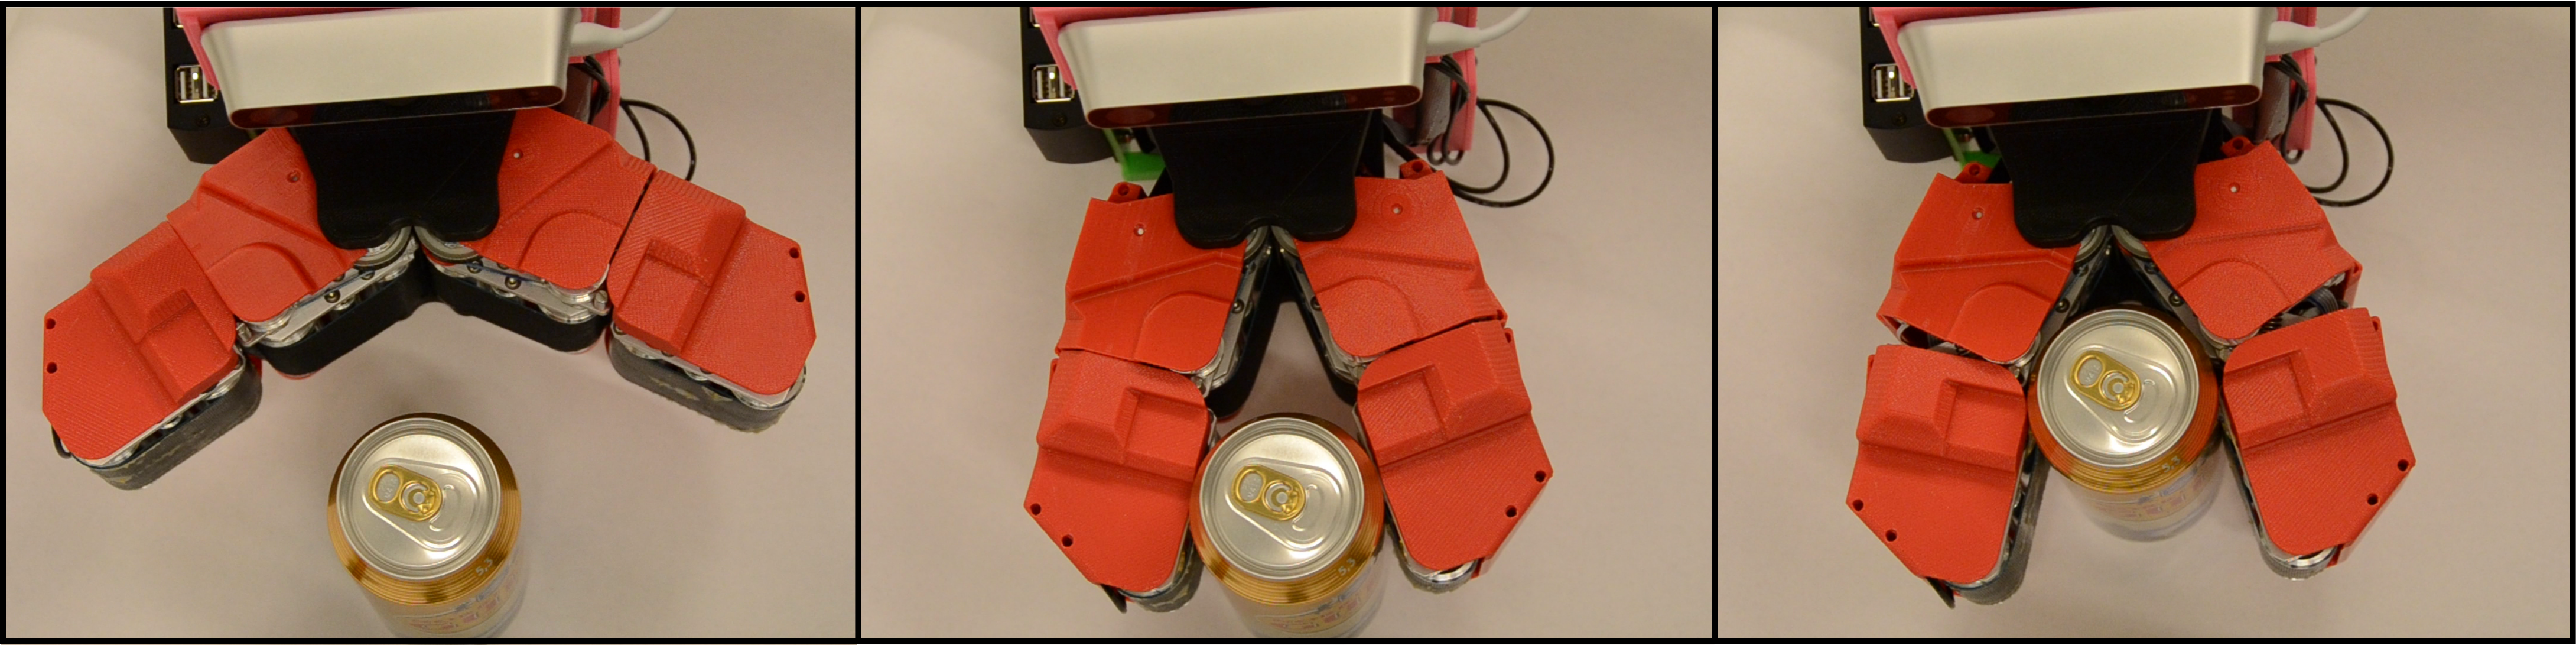
\includegraphics[width = 1.0\linewidth]{figs/pull_in}
   \caption{\textit{Pull-in grasping strategy:} Depicted is a sequence of intermediate grasp states
     where the belts of the gripper are used to pull the object towards its palm which results in a
     transition from a fingertip to an enveloping grasp.}
   \vspace{-4mm}
   \label{fig:pull_in}
   \centering
 \end{figure}
%
\begin{figure*}[!t]
 \centering
   \subfigure[]{\includegraphics[width = .32\linewidth]{figs/vcg1}}
   \subfigure[]{\includegraphics[width = .32\linewidth]{figs/vcg2}}
   \subfigure[]{\includegraphics[width = .32\linewidth]{figs/vcg3}}
   \caption{\textit{Grasp Execution Control:} As the open griper closes in on the object (Left), the
     current through the opening motor is monitored. When contact is made (Middle), the actuated
     belts are switched on to pull in the object. The controller then strives to maintain the
     current in between two target thresholds by opening or closing the gripper during in-hand
     manipulation (Right).}
   \label{fig:pull_in_control}
 \centering
\end{figure*}
%
For this component, we leverage the capabilities of the Velvet Gripper, namely underactuation and
conveyor belts on the finger pads in order to achieve robust grasping behavior. Especially in
cluttered scenes, a ``pull-in'' strategy has been shown to be especially effective to achieve stable
grasps while starting from a relatively wide range of initial gripper poses with respect to the
target object~\cite{Krug14a}. Here, the features of the grasping device are exploited to embrace the
object in a firm envelope grasp by simultaneously squeezing it in a compliant fashion while
actuating the belts inwards.

(\hl{the following is copy/pasted from the Gripper control workshop paper})~\cite{Krug14c} Each of
the gripper’s two fingers has a planar manipulator structure with two joints and active surfaces
which are implemented by coupled conveyor belts on the inside of the two phalanges. The mechanical
structure is underactuated and comprises only one actuated Degree of Freedom (DoF) for opening and
closing and two DoF for the belt movements.  If, during grasping, the proximal phalanges are blocked
by an object, the gripper’s distal phalanges continue to “wrap around” and envelope it in a firm
grasp.  The experiments reported in~\cite{Krug14a} showed, that in cluttered scenes fingertip
grasps are more likely to be feasible than robust enveloping grasps, because the latter necessitate
large opening angles resulting in bulky gripper silhouettes for which no collision free approach
trajectories can be found. Therefore, we employ the “pull-in” strategy which is illustrated in
Fig.~\ref{nothereyet}. Here, the underactuated nature and the conveyor belts on the grasping device
are exploited to embrace the object in a firm envelope grasp by simultaneously squeezing it while
actuating the belts inwards. This is achieved by compliant low-level position controllers which
saturate on experimentally evaluated current thresholds. We use a simple grasping routine which is
triggered after an initial fingertip grasp is achieved (see Fig.~\ref{nothereyet}). This routine
consists of issuing commands to fully close the gripper while moving the belts a pre-defined offset
towards the palm. Three thresholds on the current absorption of the opening motor are used: a low
threshold (LT) signifies contact between the gripper and the object and a mid threshold (MT)
indicates a large enough contact force to stop the closing movement.  Finally, an upper threshold
(UT) prevents damage to the grasping device. Once the pull-in sequence is completed, the controllers
maintain the final torques to ensure a stable grasp.

